\documentclass[twoside,a4paper]{article}
\usepackage{geometry}
\geometry{margin=1.5cm, vmargin={0pt,1cm}}
\setlength{\topmargin}{-1cm}
\setlength{\paperheight}{29.7cm}
\setlength{\textheight}{25.3cm} 

% useful packages.

\usepackage{float}
\usepackage{tikz}
\usepackage{pgfplots}
\usepackage{amsfonts}
\usepackage{amsmath}
\usepackage{amssymb}
\usepackage{amsthm}
\usepackage{enumerate}
\usepackage{multicol}
\usepackage{fancyhdr}
\usepackage{layout}
\usepackage{listings}
\usepackage{longtable}
\usepackage{multirow}
\usepackage{graphicx}
\usepackage{subfigure}
\usepackage[ruled,linesnumbered]{algorithm2e}
\usepackage{natbib}
\usepackage{mathrsfs}
\usepackage[sans]{dsfont}

% some common command
\newcommand{\dif}{\mathrm{d}}
\newcommand{\avg}[1]{\left\langle #1 \right\rangle}
\newcommand{\difFrac}[2]{\frac{\dif #1}{\dif #2}}
\newcommand{\pdfFrac}[2]{\frac{\partial #1}{\partial #2}}
\newcommand{\OFL}{\mathrm{OFL}}
\newcommand{\UFL}{\mathrm{UFL}}
\newcommand{\fl}{\mathrm{fl}}
\newcommand{\op}{\odot}
\newcommand{\Eabs}{E_{\mathrm{abs}}}
\newcommand{\Erel}{E_{\mathrm{rel}}}
\newcommand*{\circled}[1]{\hbox{\tikz\draw (0pt, 0pt)%
    circle (.5em) node {\makebox[1em][c]{\small #1}};}}

\newcommand{\mx}{{\mathbf{x}}}
\newcommand{\mX}{{\mathbf{X}}}
\newcommand{\ml}{{\mathbf{l}}}
\newcommand{\me}{{\mathbf{e}}}
\newcommand{\mb}{{\mathbf{b}}}
\newcommand{\mI}{{\mathbf{I}}}
\newcommand{\mw}{{\mathbf{w}}}
\newcommand{\mi}{{\mathbf{i}}}
\newcommand{\mj}{{\mathbf{j}}}
\newcommand{\mL}{{\mathbf{L}}}
\newcommand{\mU}{{\mathbf{U}}}
\newcommand{\mA}{{\mathbf{A}}}
\newcommand{\mP}{{\mathbf{P}}}
\newcommand{\mQ}{{\mathbf{Q}}}

\theoremstyle{definition}

\newtheorem{thm}{Theorem}[section]
\newtheorem{lem}[thm]{Lemma}
\newtheorem{prop}[thm]{Proposition}
\newtheorem{defn}[thm]{Definition}
\newtheorem{coro}[thm]{Corollary}
\newtheorem{rmk}{Remark}[section]
\newtheorem{exm}[thm]{Example}
\newtheorem{nota}[thm]{Notation}
\newtheorem{alg}[thm]{Algorithm}

\newenvironment{soln}{\paragraph{Solution.}}{\hfill\qedsymbol\null}

\newcommand{\cond}{\mathrm{cond}}

\title{Multigrid Preconditioner for Solving GePUP Equations}
\author{Liu jiyu}
\begin{document}
\maketitle

\section{GePuP Equations}
\label{sec:GePuP}

In a bounded domain $\Omega\in\mathbb{R}^D$, we numerically solve the
incompressible Navier-Stokes equations with no-slip condition:
\begin{subequations}
  \label{eq:GePuP}
  \begin{eqnarray}
  &\pdfFrac{\mathbf{w}}{t}=
  \mathbf{g}-\mathbf{u}\cdot\nabla\mathbf{u}-\nabla q +
  \nu\Delta\mathbf{w} \mbox{ in } \Omega, \\
  &\mathbf{w}=0 \mbox{ on }\partial \Omega, \\
  &\mathbf{u}=\mathscr{P}\mathbf{w}\mbox{ in } \Omega, \\
  &\mathbf{u\cdot n}=0\mbox{ on }\partial \Omega,\\
  &\Delta q =
  \nabla\cdot(\mathbf{g}-\mathbf{u}\cdot\nabla\mathbf{u})\mbox{ in
  }\Omega,\\
  &\mathbf{n}\cdot\nabla q=
  \mathbf{n}\cdot(\mathbf{g}+\nu\Delta\mathbf{u}-\nu\nabla\nabla\cdot\mathbf{u})\mbox{
  on } \partial \Omega.
\end{eqnarray}
\end{subequations}
%%% Local Variables:
%%% mode: latex
%%% TeX-master: "MGPreconditioner_MathDoc"
%%% End:

\section{Spatial Discretiazation}
\label{sec:SpatialDiscretiazation}

\begin{defn}
  $R$ is called \emph{square domain} if it can be written into
  $R=[\mathbf{x}_O,\mathbf{x}_E]$, where
  $\mathbf{x}_O,\mathbf{x}_E\in\mathbb{R}^D$.
\end{defn}
\begin{defn}
  $\Omega$ is called \emph{regular domain} if it can be written into an
  union of finite disjoint square domains, i.e.
  \begin{equation}
    \Omega = \bigcup\limits_{k=1}^NR_k,
  \end{equation}
  where $R_k$ is square domains.
\end{defn}

Let $\Omega$ be computation domain and  $R$ be a regular domain
containing $\Omega$, we discretize $R$ into a
collection of square control volumes. Denote a control colume by a multi-index
$\mathbf{i}\in \mathbb{Z}^D$, the region of cell $\mathbf{i}$ is
represented by
\begin{equation}
  \label{eq:Ci}
  C_{\mathbf{i}}=\left[\mathbf{x}_O+\mathbf{i}h,\
    \mathbf{x}_O+(\mathbf{i}+\mathds{1}h\right],
\end{equation}
and the region of the higher face of cell $\mathbf{i}$ in dimension
$d$ by
\begin{equation}
  \label{eq:Fi}
  F_{\mathbf{i}+\frac{1}{2}\mathbf{e}^d}  :=
  \left[ \mathbf{\mathbf{x}_O} + \left(\mathbf{i}+\mathbf{e}^d \right)
    h, \mathbf{x}_O
    +\left(\mathbf{i}+\mathds{1}\right)h \right],
\end{equation}
where $\mathbf{x}_O\in\mathbb{R}^D$ is some fixed origin of the
coordinates, $h$ the uniform grid size, $\mathds{1}\in\mathbb{Z}^D$
the multi-index with all its components equal to one, and
$\mathbf{e}^d\in\mathbb{Z}^D$ a multi-index with 1 as its $d$th
component and 0 otherwise.

For irregular domain $\Omega$, we embed it on a discrete square
domain and  denote the corresponding cutting control volume and
control face as
\begin{equation}
  \mathcal{C}_{\mathbf{i}}:={C}_{\mathbf{i}}\cap \Omega,\quad
  \mathcal{F}_{\mathbf{i}+\frac{1}{2}\mathbf{e}^d} :=
  {F}_{\mathbf{i}+\frac{1}{2}\mathbf{e}^d}  \cap \Omega.
\end{equation}

We call $\mathcal{C}_{\mathbf{i}}$ interior control volume if
$\mathcal{C}_{\mathbf{i}} = C_{\mathbf{i}}$, exterior control volume
if $\mathcal{C}_{\mathbf{i}}=\emptyset$, boundary control volume if
$\mathcal{C}_{\mathbf{i}}\neq C_{\mathbf{i}},\emptyset$. For a
boundary control volume, we denote its boundary as
\begin{equation}
  \label{eq:boundaryOfvolume}
  \mathcal{S}_{\mathbf{i}} := {C}_{\mathbf{i}}\cap\partial\Omega.
\end{equation}
There are the same classifications for control faces. The following
figure shows the spatial discretiazation of two different computation
domains.???

\begin{defn}
  Denote the average of a scalar function
  $\varphi:\mathbb{R}^D\rightarrow\mathbb{R}$ on a control volume
  $\mathcal{C}_{\mathbf{i}}$ as
  \begin{equation}
    \left<\varphi\right>_{\mathbf{i}} := \frac{1}{\Vert
      \mathcal{C}_{\mathbf{i}}\Vert}\int_{\mathcal{C}_{\mathbf{i}}}
    \varphi\  \mathrm{d}\mathbf{x}.
  \end{equation}
\end{defn}

\begin{defn}
  Denote the average of a scalar function
  $\varphi:\mathbb{R}^D\rightarrow\mathbb{R}$ on a control face
  $\mathcal{F}_{\mathbf{i}+\frac{1}{2}\mathbf{e}^d}$ as
  \begin{equation}
    \left<\varphi\right>_{\mathbf{i}+\frac{1}{2}\mathbf{e}^d} := \frac{1}{\Vert
      \mathcal{F}_{\mathbf{i}+\frac{1}{2}\mathbf{e}^d}\Vert}\int_{\mathcal{F}_{\mathbf{i}+\frac{1}{2}\mathbf{e}^d}}\varphi\
    \mathrm{d}\mathbf{x}.  
  \end{equation}
\end{defn}

\begin{defn}
  Denote the average of a scalar function
  $\varphi:\mathbb{R}^D\rightarrow\mathbb{R}$ on the boundary
  $\mathcal{S}_{\mathbf{i}}$ of a control volume as
  \begin{equation}
    \left[\varphi\right]_{\mathbf{i}} := \frac{1}{\Vert
      \mathcal{S}_{\mathbf{i}}\Vert}\int_{\mathcal{S}_{\mathbf{i}}}
    \varphi\  \mathrm{d}\mathbf{x}.
  \end{equation}
\end{defn}


There are three cases when discretize operators:
\begin{enumerate}
\item For the control volumes or faces in $\Omega$ which are far away
  from the boundary, we use standard finite volume stencils.
\item For the control volumes or faces near the regular boundary, we
  fill the ghost cells with boundary conditions and then use standard
  finite volume formulae.
\item For the control volumes or faces near the irregular boundary, we
  generate a poised lattice by poised lattice
  generating algorithm, then fit a complete
  multivariate polynomial with the poised lattice to obtain the
  discretized equation.
\end{enumerate}

\subsection{Standard finite difference formulae}
\label{sec:Standard}

In the regular domain, the discrete gradient, the discrete divergence and the dicrete
Laplacian are
\begin{eqnarray}
  \label{eq:G}
  \mathbf{G}_d\left<\phi\right>_{\mathbf{i}} &:=&
  \frac{1}{12h}\left(-\left<\phi\right>_{\mathbf{i}+2\mathbf{e}^d}
    +8\left<\phi\right>_{\mathbf{i}+\mathbf{e}^d}
    -8\left<\phi\right>_{\mathbf{i}-\mathbf{e}^d} 
  +\left<\phi\right>_{\mathbf{i}-2\mathbf{e}^d}\right) \\
  \label{eq:D}
  \mathbf{D}\left<\mathbf{u}\right>_{\mathbf{i}} &:=&
  \frac{1}{12h}\sum\limits_d \left( -\left<u_d\right>_{\mathbf{i}+2\mathbf{e}^d}
    +8\left<u_d\right>_{\mathbf{i}+\mathbf{e}^d}
    -8\left<u_d\right>_{\mathbf{i}-\mathbf{e}^d} 
                                                      +\left<u_d\right>_{\mathbf{i}-2\mathbf{e}^d}\right) \\
  \label{eq:L}
  \mathbf{L}\left<\phi\right>_{\mathbf{i}} &:=&
  \frac{1}{12h^2}\sum\limits_d\left(-\left<\phi\right>_{\mathbf{i}+2\mathbf{e}^d}
    +16\left<\phi\right>_{\mathbf{i}+\mathbf{e}^d} - 30\left<\phi\right>_{\mathbf{i}} 
    +16\left<\phi\right>_{\mathbf{i}-\mathbf{e}^d} 
  -\left<\phi\right>_{\mathbf{i}-2\mathbf{e}^d}\right) \\
\end{eqnarray}

The discrete divergence also acts on tensor averages
\begin{equation}
  \label{eq:Duu}
  \mathbf{D}\left<\mathbf{uu}\right>_{\mathbf{i}} :=
  \frac{1}{h}\sum\limits_d\left(
    \mathbf{F}\left<u_d,\mathbf{u}\right>_{\mathbf{i}+\frac{1}{2}\mathbf{e}^d}
    -
    \mathbf{F}\left<u_d,\mathbf{u}\right>_{\mathbf{i}-\frac{1}{2}\mathbf{e}^d}  \right),
\end{equation}
where the average of the product of two scalars over a cell face is
\begin{equation}
  \label{eq:ProductOf2scalar}
  \mathbf{F}\left<\phi,\psi\right>_{\mathbf{i}+\frac{1}{2}\mathbf{e}^d}
  :=
  \left<\phi\right>_{\mathbf{i}+\frac{1}{2}\mathbf{e}^d}
  \left<\psi\right>_{\mathbf{i}+\frac{1}{2}\mathbf{e}^d}+
  \frac{h^2}{12}\sum\limits_{d'\neq
    d}\left(\mathbf{G}^{\perp}_{d'}\phi\right)_{\mathbf{i}+\frac{1}{2}\mathbf{e}^d}
  \left(\mathbf{G}^{\perp}_{d'}\psi\right)_{\mathbf{i}+\frac{1}{2}\mathbf{e}^d},
\end{equation}
and $\mathbf{G}^{\perp}_{d'}$ is the discrete gradient in the
transverse directions
\begin{equation}
  \label{eq:TransverseG}
  \left(\mathbf{G}^{\perp}_{d'}\phi\right)_{\mathbf{i}+\frac{1}{2}\mathbf{e}^d}
  :=
  \frac{1}{2h}\left(\left<\phi\right>_{\mathbf{i}+\frac{1}{2}\mathbf{e}^d+\mathbf{e}^{d'}}-
  \left<\phi\right>_{\mathbf{i}+\frac{1}{2}\mathbf{e}^d-\mathbf{e}^{d'}}
 \right)
\end{equation}

$\mathbf{G}\left<\phi\right>,\ \mathbf{D}\left<\mathbf{u}\right>,\
\mathbf{L}\left<\mathbf{u}\right>$ and 
$\mathbf{D}\left<\mathbf{uu}\right>$ approximate the cell average of a
gradient, velocity divergence, Laplacian, and convection,
respectively. These discrete operators are fomally fourth-order
accurate in approximating their continuous counterparts.[?]

\subsection{Ghost Cell}
\label{sec:GhostCell}

Following ?, two layers of ghost cells are used to enforce boundary
conditions.  For nonperiodic boundaries, the values of ghost cells are
obtained by extrapolating those of the interior cells, with the
boundary conditions incorporated in the extrapolation formulas. For
example, homogeneous Dirichlet boundary conditions for a scalar $\psi$
are fulfilled by filling the ghost cells with the following
fifth-order formulas:
\begin{equation}
  \label{eq:GhostedDiri}
  \begin{aligned}
    \left<\psi\right>_{\mathbf{i}+\mathbf{e}^d} = \frac{1}{12}\left(
      -77\left<\psi\right>_{\mathbf{i}} +
      43\left<\psi\right>_{\mathbf{i}-\mathbf{e}^d} -
      17\left<\psi\right>_{\mathbf{i}-2\mathbf{e}^d} +
      3\left<\psi\right>_{\mathbf{i}-3\mathbf{e}^d}\right) + O(h^5), \\
    \left<\psi\right>_{\mathbf{i}+2\mathbf{e}^d} = \frac{1}{12}\left(
      -505\left<\psi\right>_{\mathbf{i}} +
      335\left<\psi\right>_{\mathbf{i}-\mathbf{e}^d} -
      145\left<\psi\right>_{\mathbf{i}-2\mathbf{e}^d} +
      27\left<\psi\right>_{\mathbf{i}-3\mathbf{e}^d}\right) + O(h^5),
  \end{aligned}
\end{equation}
Neumann boundary conditions are fulfilled by
\begin{equation}
  \label{eq:GhostedNeumann}
  \begin{aligned}
    \left<\psi\right>_{\mathbf{i}+\mathbf{e}^d} = \frac{1}{10}\left(
      5\left<\psi\right>_{\mathbf{i}} +
      9\left<\psi\right>_{\mathbf{i}-\mathbf{e}^d} -
      5\left<\psi\right>_{\mathbf{i}-2\mathbf{e}^d} +
      \left<\psi\right>_{\mathbf{i}-3\mathbf{e}^d}\right) +
    \frac{6}{5}h\left<\pdfFrac{\psi}{n}\right>_{\mathbf{i}+\frac{1}{2}\mathbf{e}^d} + O(h^5), \\
    \left<\psi\right>_{\mathbf{i}+2\mathbf{e}^d} = \frac{1}{10}\left(
      -75\left<\psi\right>_{\mathbf{i}} +
      145\left<\psi\right>_{\mathbf{i}-\mathbf{e}^d} -
      75\left<\psi\right>_{\mathbf{i}-2\mathbf{e}^d} +
      15\left<\psi\right>_{\mathbf{i}-3\mathbf{e}^d}\right) +
    6h\left<\pdfFrac{\psi}{n}\right>_{\mathbf{i}+\frac{1}{2}\mathbf{e}^d}
    + O(h^5),
  \end{aligned}
\end{equation}
where
$\left<\pdfFrac{\psi}{n}\right>_{\mathbf{i}+\frac{1}{2}\mathbf{e}^d} $
is the Neumann condition for $\psi$. 

\subsection{PLG}
\label{sec:PLG}

For the control volumes and faces near the irregular boundary, where
we can not use standard difference formulae, our idea is:
\begin{enumerate}
\item Clarify the control volume $\mathcal{C}_{\mathbf{i}}$ (or
  control face $\mathcal{F}_{\mathbf{i}+\frac{1}{2}\mathbf{e}^d}$)
  where differential operator $\mathcal{L}$ is discretized, order of
  spatial discretiazation $p$, and the average of differential
  operator on control volumes 
  $\left\{\left<\varphi\right>_{\mj}:\mj\in\mathbb{Z}^D\right\}$ (or
  on control faces
  $\left\{\left<\varphi\right>_{\mj}:\mj\in\mathbb{Z}^D+\frac{1}{2}\me^d\right\}$
  ).
\item As shown in Figure ?, we calculate finite volume stencil of
  $\left<\mathcal{L}\varphi\right>_{\mi}$ with poised lattice
  generating algorithm, denote it as
  \begin{equation}
    \label{eq:Stencil}
    \mathcal{X}(\mi) =
    \{\mathcal{C}_{\mj_1},\cdots,\mathcal{C}_{\mj_N}\} \cup
    \{\mathcal{S}_{\mj_{N+1}},\cdots,\mathcal{S}_{\mj_{N+N'}}\}
  \end{equation}
  where $N=\dim\Pi_n^D$, $n=p+q-1$ is the order of stencil, $q$ is the
  order of differential operator, $N'$ is the number of boundry terms.
\item Fit a complte multivariate polynomial with the finite volume
  stencil $\mathcal{X}(\mi)$:
  \begin{equation}
    \label{eq:FittingPoly}
    p(\mx)=\sum\limits_{j=1}^N \alpha_j\phi_j(\mx)\in\Pi_n^D,
  \end{equation}
  where $\left\{\phi_j\right\}_{j=1}^N$ is a basis of $\Pi_n^D$,
  coefficient $\mathbf{\alpha} = [\alpha_1,\cdots,\alpha_n]^T$ is the
  solution of weighted least squares problem
  \begin{equation}
    \label{eq:WeightedLSP}
    \min_{\alpha}\sum_{k=1}^N\omega_k\left|\left<p\right>_{\mj_k} -
      \varphi_k\right|^2 +
    \sum_{k=N+1}^{N=N'}\omega_k\left|\left[\mathcal{N}p\right]_{\mj_k} -
    \varphi_k\right|^2,
  \end{equation}
  where weight $\omega_k$ depends on the relative position of
  $\mathcal{C}_{\mj_k}$ and $\mathcal{C}_{\mi}$.
\item Finally discretize the differential operator with fitted
  polynomial \eqref{eq:FittingPoly}:
  \begin{equation}
    \label{eq:DiscreteOp}
    \left<\mathcal{L}\varphi\right>_{\mi} =
    \left<\mathcal{L}p\right>_{\mi}  + O(h^p) =
    \sum_{k=1}^N\beta_k\left<\varphi\right>_{\mj_k}+
    \sum_{k=N+1}^{N+N'}\beta_k\left[\mathcal{N}\varphi\right]_{\mj_k} + O(h^p).
  \end{equation}
\end{enumerate}

Above all, we obtain the spatial discretization of GePuP equations
\eqref{eq:GePuP}:
\begin{subequations}
  \label{eq:SemiGePuP}
  \begin{eqnarray}
  &\frac{\mathrm{d}\left<\mathbf{w}\right>}{\mathrm{d}t}=
  \left<\mathbf{g}\right>-\mathbf{D}\left<\mathbf{uu}\right>
    -\mathbf{G}\left<q\right> +
    \nu\mathbf{L}\left<\mathbf{w}\right> \mbox{ in } \Omega,
    \label{eq:SemiGePuPa}\\
  &\left[\mathbf{w}\right]=0 \mbox{ on }\partial \Omega, \\
  &\left<\mathbf{u}\right>=\mathbb{P}\left<\mathbf{w}\right>\mbox{ in
    } \Omega, \\
  &\left[\mathbf{u\cdot n}\right]=0\mbox{ on }\partial \Omega,\\
  &\mathbf{L}\left<q\right> =
  \mathbf{D}(\left<\mathbf{g}\right>-\mathbf{D}\left<\mathbf{uu}\right>)
    \mbox{ in }\Omega,\\
  &\left[\mathbf{n}\cdot\nabla q\right]=
  \left[\mathbf{n}\cdot\mathbf{g}\right]+\nu\left[(\mathbf{n}\cdot\mathbf{L})\mathbf{u}\right]-\nu\left[(\mathbf{n\cdot
    G})\mathbf{D}\mathbf{u}\right]\mbox{
  on } \partial \Omega.
\end{eqnarray}
\end{subequations}
with the initial conditions
\begin{subequations}
  \label{eq:SemiGePuPInitialCond}
  \begin{eqnarray}
    &\left<\mathbf{u}\right>(t_0)=\left<\mathbf{w}\right>(t_0),\\
    &\left[\mw\right]=\mathbf{0}.
  \end{eqnarray}
\end{subequations}
Now we obtain the fourth-order (spatial) semi-discrete formulae of
GePuP for incompressible Navier-Stokes equations.


%%% Local Variables:
%%% mode: latex
%%% TeX-master: "MGPreconditioner_MathDoc"
%%% End:


\section{Time Integration}
\label{sec:TimeIntegration}

We apply ERK-ESDIRK to semi-discrete formulae \eqref{eq:SemiGePuP}, in
which the RHS of \eqref{eq:SemiGePuPa} is divided into an explicit
part and an implicit part:
\begin{subequations}
  \begin{eqnarray}
    &\mathbf{X}^{[E]} = \left<\mathbf{g}\right>-\mathbf{D}\left<\mathbf{uu}\right>
      - \mathbf{G}\left<q\right>, \\
    & \mathbf{X}^{[I]} = \nu\mathbf{L}\left<\mw\right>.
  \end{eqnarray}
\end{subequations}

Now we obtain GePuP-IMEX algorithm:
\begin{subequations}
  \begin{eqnarray}
    &&\left<\mathbf{w}\right>^{(1)}=\left<\mathbf{w}\right>^{n}, \\
    &&\left\{
    \begin{array}{l}
      \mbox{for } s=2,3,\cdots,n_s, \\
      \left(\mathbf{I}-\Delta
      t\gamma\nu\mathbf{L}\right)\left<\mathbf{w}\right>^{(s)} =
      \left<\mathbf{w}\right>^{n} + \Delta
      t\sum\limits_{j=1}^{s-1}a_{s,j}^{[E]}\mX
      ^{[E]}\left(\left<\mathbf{u}\right>^{(j)},t^{(j)}\right) +\Delta
      t\nu\sum\limits_{j=1}^{s-1}a_{s,j}^{[I]}\mL\left<\mathbf{w}\right>^{(j)},\\
      \left<\mathbf{u}\right>^{(s)}=\mathbb{P}\left<\mathbf{w}\right>^{(s)},
    \end{array} 
    \right.\\
    &&\left\{
       \begin{array}{l}
         \left<\mathbf{w}\right>^*=\left<\mathbf{w}\right>^{(n_s)}+\Delta
         t\sum\limits_{j=1}^{n_s}\left(b_j-a_{n_s,j}^{[E]}\right)\mX^{[E]}\left(\left<\mathbf{u}
         \right>^{(j)},t^{(j)}\right),\\
         \left<\mathbf{u}\right>^{n+1}=\mathbb{P}\left<\mathbf{w}\right>^*,\\
         \left<\mathbf{w}\right>^{n+1}=\left<\mathbf{u}\right>^{n+1}.
       \end{array}
       \right.
  \end{eqnarray}
\end{subequations}

There are three linear systems of equations need to be solved at each
intermediate stage:
\begin{enumerate}
\item A Poisson equation with Neumann boundary condition for
  extracting $\left<q\right>$ from $\left<\mathbf{u}\right>$.
\item A Helmholtz equation with no-slip boundary condition for
  evaluating $\left<\mathbf{u}\right>$.
\item A Poisson equation with Neumann boundary condition for
  projecting $\left<\mw\right>^*$.
\end{enumerate}

Above all, the essence of our work is solving a Poisson equation
$L\phi=b$ on
an irregular domain, the spatial discretization is  the same as that
in section \ref{sec:SpatialDiscretiazation}.

%%% Local Variables:
%%% mode: latex
%%% TeX-master: "MGPreconditioner_MathDoc"
%%% End:


\section{The multigrid preconditioned Krylov methods}
\label{sec:MGPre}

We concentrate on the system of discrete equations
\begin{equation}
  \label{eq:AX=B}
  \mA\mx=\mb,
\end{equation}

Matrix $\mA$ has right preconditioning as follows:
\begin{equation}
  \label{eq:RightPre}
  \mathbf{AK}^{-1}(\mathbf{Kx})=\mb.
\end{equation}
The preconditioned Krylov subspace methods are used for solving
\eqref{eq:RightPre}, such as BiCGSTAB and GMRES($m$).

\begin{alg}
  The GMRES($m$) algorithm with a right multigrid preconditioner
  appears as follows:

 \IncMargin{1em}
 \LinesNumbered
 \begin{algorithm}[H]
   \SetKwInOut{Precond}{Preconditions}
   \SetKwInOut{Postcond}{Postconditions}

   \caption{\texttt{GMRES($m,A,b,x,\epsilon$)}}
   \KwIn{$m\in\mathbb{Z}^+$, $A\in\mathbb{R}^{N\times N}$,
     $b\in\mathbb{R}^n$, $x\in\mathbb{R}^n$, 
     $\epsilon\in\mathbb{R}^+$.
     .}
   \KwOut{The solution which overwrites $x$.}
   \BlankLine
   Choose $x^{(0)}=x$, dimension $m$. matrix $\mathbf{H}=\mathbf{0}$
   with dim: $(m+1)\times m$\;
   $r^{(0)}=b-Ax^{(0)},\ \beta=\Vert r\Vert_2^2,\ f_1=r^{(0)}/\beta$\;
   \For{$j=1,\cdots,m$}{
     $u_j=K^{-1}f_j$\;
     $w=Au_j$\;
     \For{$i=1,\cdots,j$}{
       $h_{i,j}=(w,f_i)$\;
       $w = w - h_{i,j}f_j$\;
       $h_{j+1,j} = \Vert w \Vert_2$\;
       $f_{j+1} = w/h_{j+1,j}$\;
     }
   }
   Define $\mathbf{F}_m := [f_1,\cdots,f_m]$\;
   $x^{(m)}:=x^{(0)} + K^{-1}\mathbf{F}_my_m$ with $y_m=\min_y\Vert
   \beta e_1-\mathbf{H}y \Vert_2$\;
   Compute $r^{(m)}=b-Ax^{(m)}$\;
   \If{$\vert r^{(m)} \Vert_2 < \epsilon\Vert b \Vert_2$}{
     \textbf{Stop.}
   }\Else{
     restrart with $x^{(0)}\leftarrow x^{(m)}$\;
   }
 \end{algorithm}
 \DecMargin{1em}
 In line $4$, $K^{-1}f_j$ is the preconditioning step, which is one
 iteration of a multigrid cycle.
\end{alg}

The following theorem is an estimation of the convergence of
GMRES($m$) in cases where most of the eigenvalues (the last $n-l$
eigenvalues in the theorem below) of the preconditioned matrix
$\tilde{A}$ are close to $1\in\mathbb{C}.$

\begin{thm}
  \label{thm:GMRES}
  Let $\tilde{A}$ be an $n\times n$ nonsingular matrix with
  eigenvalues $\left\{\lambda_i\in\mathbb{C}\ |\  1\leq i \leq n\right\}$,
  $\overline{V}_l$ be the subspace spanned by the vectors
  $\left\{ v\ |\ \prod_{k>l}^n(\lambda_kI-\tilde{A})v=0\right\}$,
  $K_l$ be the Krylov subspave
  $K(l,r^{(0)},\tilde{A})=\mbox{span}\left\{ r^{(0)},
    \tilde{A}r^{(0)},\cdots, \tilde{A}^{l-1}r^{(0)}\right\}$, 
  $P_k$ be a set of $k$th-order complex polynomials $p_k(\lambda)$ that
  satisfy $p_k(0)=1$, and $r^{(0)}=b-\tilde{A}x^{(0)}$ be the initial
  residual. Define radius $\Gamma_i$ as
  \begin{equation}
    \label{eq:Radius}
    \Gamma_i := \max\left\{\Vert (\lambda_iI-\tilde{A})v \Vert_2\ |\ 
      v\in\overline{V}_{i-1}\cap K_i, \Vert v \Vert_2=1\right\}.
  \end{equation}
  Then a vector $\overline{r}^{(l)}$ defined by
  \begin{equation}
    \label{eq:rl}
    \overline{r}^{(l)} :=
    \left(\prod\limits_{i=1}^l\frac{1}{\lambda_i}(\lambda_iI-\tilde{A})\right)r^{(0)}
  \end{equation}
  is included in $\overline{V}_l\cap K_{l+1}.$

  Furthermore,
  \begin{equation}
    \label{eq:normOfrRl}
    \Vert \overline{r}^{(l)} \Vert_2 \leq
    \left(\prod\limits_{i=1}^l\frac{\Gamma_i}{|\lambda_i|}\right)
    \Vert r^{(0)}\Vert_2.
  \end{equation}
  Assuming $l<k\leq m$, then the norm of the residual of $k$th
  GMRES($m$) iteration can be estimated as follows:
  \begin{eqnarray}
    \label{eq:normOfResidual}
    \Vert r^{(k)} \Vert_2&\leq& \min\left\{\Vert
    p_{k-l}(\tilde{A})r^{(l)}\Vert_2 \ |\  p_{k-l}(\lambda)\in P_{k-l}\right\}
    \\
    \label{eq:normOfResidual2}
                         &\leq& \Vert (I-\tilde{A})^{k-l}\overline{r}^{(l)} \Vert_2.
  \end{eqnarray}
\end{thm}

According to Theorem \ref{thm:GMRES}, if some eigenvalues
$\lambda_i(i\leq l)$ are close to zero, the norm of
$\overline{r}^{(l)}$ becomes large. This suggests that we may need a
relatively large $k$ to reduce the residual by a certain order of
magnitude even if $l$ is not large.

Inequality \eqref{eq:normOfResidual} shows that $\Vert r^{(k)}
\Vert_2$ is not larger than the norm of the $(k-l)$th residual of
GMRES($m$) with initial residual $\overline{r}^{(l)}$ that is included
in the subspace corresponding to the eigenvalues close to one
$\left\{\lambda_i\ |\ i>l\right\}$.

Backtrack to the multigrid preconditioner, an iteration of a multigrid
cycle is equivalent to a Richardson iteration on  the preconditioned
matrix\cite{oosterlee_evaluation_1998}. With $K$ being the iteration
matrix, multigrid
can be written as follows:
\begin{equation}
  \label{eq:RichardsonIter}
  Kx^{(k+1)}+(A-K)x^{(k)}=b.
\end{equation}

If we use multigrid solver, the formulation is equivalent to
\begin{equation}
  \label{eq:Richardson2}
  x^{(k+1)} = x^{(k)} + K^{-1}(b-Ax^{(k)}) = x^{(k)}+K^{-1}r^{(k)};\
  r^{(k+1)} = (I-AK^{-1})r^{(k)}.
\end{equation}

The spectral radius of $I-AK^{-1}$ determines the convergence of
multigrid solver. With
this spectrum we can also investigate the convergence of
preconditioned GMRES method. From \eqref{eq:normOfResidual2}, the asymptotic
convergence of GMRES($m$) is at least faster than Richardson with an initial
residual. 

In \cite{oosterlee_evaluation_1998}, the author compared multigrid preconditioned
GMRES($m$) and multigrid solver in several singularly perturbed
problems. In \cite{guy_multigrid_2012}, the author compared multigrid
preconditioned GMRES($m$) and multigrid solver for implicit immersed
boundary equations. Here is an example:

\begin{exm}
  Here is a rotated anisotropic diffusion problem:
  \begin{equation}
    \label{eq:RotatingCon-D}
    -(\cos^2\beta +\epsilon\sin^2\beta)\frac{\partial^2\phi}{\partial
      x^2} - 2(\epsilon -
    1)\cos\beta\sin\beta\frac{\partial^2\phi}{\partial x\partial y} -
    (\epsilon\cos^2\beta + \sin^2\beta)\frac{\partial^2\phi}{\partial
      y^2} = 1
    \mbox{ on } \Omega=(0,1)\times (0,1).
\end{equation}
Here $\epsilon=10^{-5}$, $\beta=135^o$ and boundary conditions are prescribed :
\begin{equation}
  \begin{aligned}
    \pdfFrac{\phi}{n} = 0 \mbox{ on } \{x=0,\ 0\leq y\leq 1\},\{0\leq
    x\leq 1,\ y=0\},\\
    \phi=0\mbox{ on } \{x=1,\ 0\leq y\leq 1\},\{0\leq x\leq 1,\ y=1\}.
  \end{aligned}
\end{equation}

For this test problem, the eigenvalue spectrum of the Richardson
iteration matrix $I-AK^{-1}$ is investigated on a $33\times 33$ grid,
as presented in figure \ref{fig:spectrum}.

\begin{figure}[htbp]
      \centering
      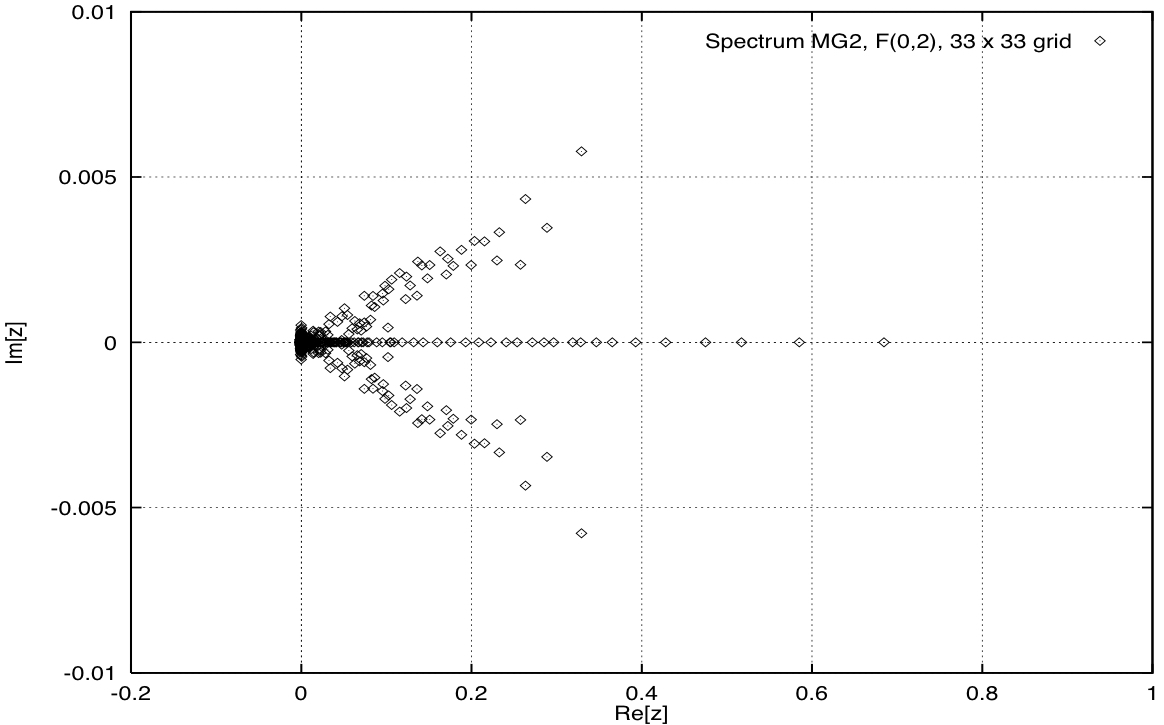
\includegraphics[width=0.5\textwidth]{Spectrum.png}
      \caption{The eigenvalue spectra for the rotated anisotropic
        diffusion problem,$\epsilon=10^{-5}$, $\beta=135^o$ on a
        $33\times 33$ grid.}
      \label{fig:spectrum}
    \end{figure}

It can be seen that the spectral radius for coarse grid problems is
already larger than 0.6. Therefore, the multigrid convergence slows
down more dramatically than the convergence of the preconditioned
Krylov methods. What's more, eigenvalues of the preconditioned matrix
$(AK^{-1})$ are clusted around $1$, which is advantageous for the
Krylov methods. The convergence of multigrid as solution methods and
as preconditioners for GMRES(20) is presented for $33\times 33$ grid
in Figure \ref{fig:convergence}.

\begin{figure}[htbp]
      \centering
      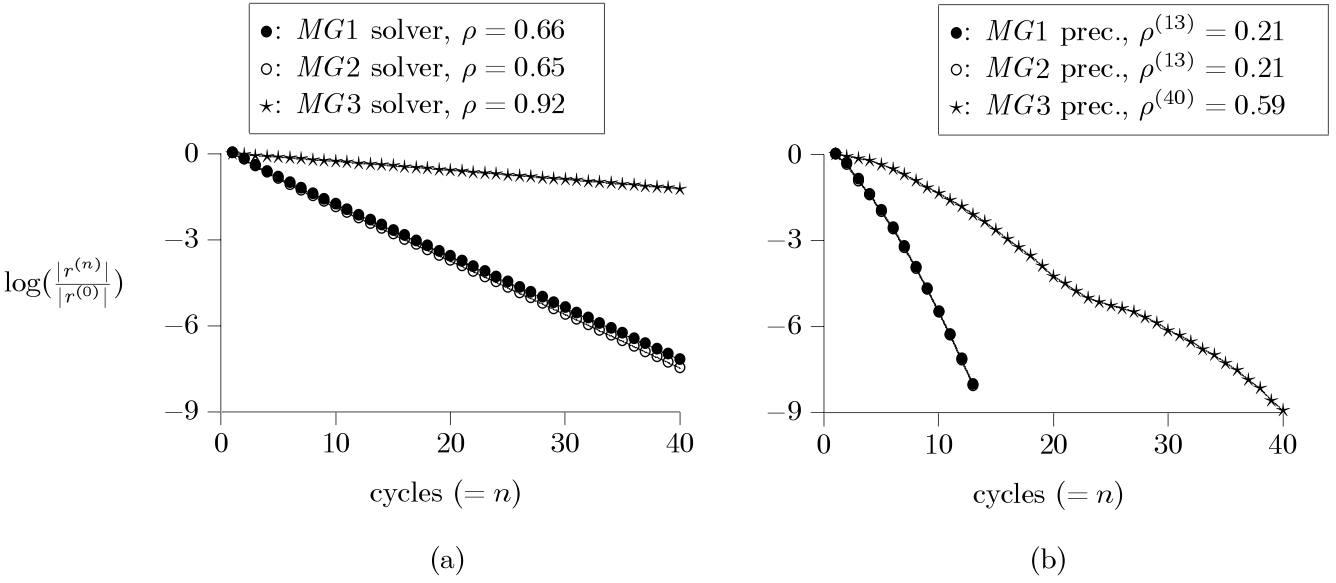
\includegraphics[width=0.75\textwidth]{Convergence.png}
      \caption{The convergence of the MG solvers (a), GMRES(20)
        with MG preconditioners (b) for the rotated anisotropic
        diffusion equation on a $33\times 33$ grid.}
      \label{fig:convergence}
    \end{figure}

MG1, MG2, MG3 are multigrid methods with different prolongation and
restriction operators. It can be seen that different prolongation and
restriction operators will affect the convergence rate. However, no
matter which operators are used, MG preconditioned GMRES($m$) method
performs better than MG solver in this problem.
\end{exm}



The conclusion is that the behaviors of the multigrid methods
are much more robust when they are used as preconditioners, problems
that could not be solved with the multigrid methods as solvers could
be solved with the preconditioned Krylov methods. The efficiency of
the multigrid solver alone is not impressive, but it is a very
effective preconditioner for Krylov methods. We also can improve the
preconditioned Krylov methods by using a more sophisticated smoother
in multigrid preconditioner, just like Figure \ref{fig:convergence}.

\section{Next step}
\label{sec:goal}

The follow-up work is mainly divided into two steps:

\begin{enumerate}
\item There is not much mathematical theory on multigrid
  preconditioned Krylov subspace methods, most papers do numerical
  experience to compare multigrid solver and multigrid preconditioner.
  So firstly we could investigate the eigenvalue spectrum of the
  Richardson iteration matrix $I-AK^{-1}$ in
  \eqref{eq:Richardson2} of three linear systems during solving GePuP
  equations. If many eigenvalues are clustered around zero and only a
  limited number of eigenvalues are far from zero, eigenvalues of the preconditioned
  matrix $AK^{-1}$  will be clustered around one, which is
  advantageous for the Krylov methods by Theorem \ref{thm:GMRES}.
\item Then implement multigrid preconditioned GMRES($m$) method,
  apply it to solve GePuP equations, and compare it with the original program
  in terms of convergence and efficiency.
\end{enumerate}



%%% Local Variables:
%%% mode: latex
%%% TeX-master: "MGPreconditioner_MathDoc"
%%% End:

\bibliography{ref.bib}
\bibliographystyle{abbrvnat}
\setcitestyle{authoryear,open={[},close={]}}

 \end{document}
%%% Local Variables:
%%% mode: latex
%%% TeX-master: t
%%% End:
